\documentclass[a4paper,12pt]{article}
\usepackage[utf8]{inputenc}
\usepackage{amsmath}
\usepackage{amsfonts}
\usepackage{amssymb}
\usepackage{graphicx}
\usepackage{caption}
\usepackage{subcaption}
\usepackage{float}
\usepackage{siunitx}
\usepackage{booktabs}
\usepackage{hyperref}

\title{Rapporto carica-massa dell'elettrone}
\author{Francesco Giuseppe Minisini, Mattia Monzani, Gabriele Turi}
\date{January 13, 2025}

\begin{document}

\maketitle
\hrule
\vspace{9pt}
\begin{abstract}
    \noindent
    In questa relazione viene documentata la misura del rapporto carica-massa dell'elettrone \(\frac{e}{m}\) tramite l'osservazione della traiettoria circolare descritta dagli elettroni all'interno di un campo magnetico generato da bobine in configurazione di Helmholtz. Le misure sono state effettuate in tre configurazioni distinte rispetto al campo magnetico terrestre: ortogonale \((1.75 \pm 0.17) \times 10^{11} \, \text{C/kg}\), antiparallela \((1.79 \pm 0.20) \times 10^{11} \, \text{C/kg}\) e parallela \((1.95 \pm 0.20) \times 10^{11} \, \text{C/kg}\). Dopo aver misurato il campo magnetico terrestre tramite osservazione dell'effetto su una bussola e ottenuto il valore \(B_T = (24.6 \pm 0.4) \, \mu\text{T}\), il contributo di quest'ultimo è stato corretto, migliorando la compatibilità dei risultati con il valore teorico di \(1.7588 \times 10^{11} \, \text{C/kg}\).
    
\vspace{20pt}
\hrule
\end{abstract}
\vspace{2 pt}


\section{Descrizione dell’apparato sperimentale}
Per la misura del rapporto carica-massa dell’elettrone, è necessario accelerare e visualizzare il moto degli elettroni all’interno di uno specifico apparato. 
Lo studio del moto degli elettroni avviene all’interno di una sfera di vetro di riempita di molecole diatomiche di idrogeno ad una pressione di \(10^{-2} \, \text{torr}\). La collisione tra un elettrone e una molecola di idrogeno comporta l’eccitazione di quest’ultima che viene accompagnata da l’emissione di fotoni luminosi. Dunque, grazie all’urto tra l’elettrone e le molecole di idrogeno è possibile visualizzare una scia di colore azzurro che consente quindi di osservare il cammino degli elettroni. Con una pressione per l’appunto di \(10^{-2} \, \text{torr}\) il gas presente nella sfera di vetro è sufficientemente rarefatto affinché il cammino medio di ogni elettrone, prima di collidere con una molecola di idrogeno, sia sufficientemente elevato da visualizzare una scia completa. All’interno della sfera, lungo un circuito penetrante nella sfera, è inserito un filamento metallico di tungsteno, in grado di essere scaldato dal circuito, alimentato a corrente alternata con una tensione di \(4 \, \text{Volt}\), per “effetto Joule”. Il filamento è presente all’interno di una struttura metallica a forma di tronco di cono che presenta un catodo nell’estremità inferiore, poggiante sopra il filamento riscaldato, e un anodo all’estremità superiore, dotata di un beccuccio forato per rendere possibile la fuoriuscita di elettroni. Il catodo viene riscaldato per contatto con il filamento tungsteno, il che causa la fuoriuscita di alcuni elettroni presenti sul catodo per “effetto termo-elettronico”. A questo punto, un secondo circuito, alimentato a corrente continua e con tensioni tra i \(150 \, \text{Volt}\) e i \(300 \, \text{Volt}\), collegato al catodo e all’anodo, accelera gli elettroni verso l’alto attraverso il beccuccio forato dell’anodo, da cui fuoriescono e consentono la visualizzazione della traiettoria nell’ampolla. (Gli elettroni, una volta accelerati e fuori usciti dal foro, non essendo più soggetti a forze non trascurabili, compiono una traiettoria rettilinea, verticalmente verso l’alto). Per la determinazione del rapporto carica-massa dell’elettrone si vuole procede con lo studiare moto degli elettroni soggetti alla “forza di Lorentz” che essi avvertono in presenza di un campo magnetico esterno. Il campo magnetico esterno nell’esperimento viene generato tramite bobine conduttrici attraversate da corrente elettrica, in mezzo alle quali viene posta la sfera. Le due bobine utilizzate, composte da 130 spire, sono state disposte secondo la “configurazione di Helmholtz”, che prevede il parallelismo tra le due bobine e che la distanza che le separa sia pari al loro raggio medio. Tale configurazione permette la generazione, tra le due bobine, di un campo magnetico parallelo al suolo, e ortogonale alle due bobine, il più approssimativamente uniforme possibile. La forza di Lorentz a cui sono soggetti gli elettroni, essendo, come noto, ortogonale alla velocità degli elettroni, incurva il moto degli elettroni, che compiono così un moto circolare; pertanto, la scia visibile all’interno della sfera assume una forma circolare. 
Nell’esperimento condotto è stata in seguito anche effettuata la misura del campo magnetico terrestre. Questa misurazione è stata eseguita tramite un apparato composto da una piattaforma, dotata di un ago magnetico e di goniometro graduato per la misurazione dell’orientazione dell’ago, interposta tra due bobine conduttrici, dalla geometria nota e alimentabili con corrente, disposte l’una di fronte l’altra e con asse lungo la direzione orizzontale. 

\section{Misurazione del rapporto carica-massa dell’elettrone}
Per misurare il rapporto carica-massa dell’elettrone con questo apparato è necessario prima individuare quali sono le grandezze da misurare.
Tramite considerazioni energetiche, in particolare applicando il teorema dell’energia cinetica, si stima che l’elettrone, di massa \( m \) e carica \( e \), venga accelerato dalla differenza di potenziale \( \Delta V \) presente tra catodo e anodo fino ad una velocità \( v \), tale che:

\begin{equation}
    \frac{e}{m} = \frac{1}{2} \frac{v^2}{\Delta V}
    \label{eq:rapporto_carica_massa}
\end{equation}
Dunque, la differenza di potenziale \( \Delta V \) tra catodo e anodo è una delle grandezze da misurare.
Per esprimere la velocità dell’elettrone in funzione di altre grandezze che siano più agevolmente misurabili con gli strumenti di misura a disposizione, si pone l’espressione nota della forza di Lorentz uguale all’espressione di una forza centripeta, siccome nell’esperimento la forza di Lorentz dovuta al campo magnetico di intensità \( B \) fa compiere agli elettroni un moto circolare uniforme di raggio \( R \). Da cui si ottiene:

\begin{equation}
    \frac{e}{m} = \frac{2 \Delta V}{B^2 R^2}
    \label{eq:forza_lorentz}
\end{equation}

Pertanto, le altre due grandezze da misurare sono il raggio della traiettoria circolare degli elettroni e il campo magnetico generato dalle bobine, esprimibile in funzione del raggio delle bobine \( R_b \) e dell’intensità di corrente \( I \) che scorre nei fili delle bobine, misurabili direttamente dagli strumenti forniti in dotazione in laboratorio, utilizzando la seguente relazione:

\begin{equation}
    B = \mu_0 \frac{8NI}{5\sqrt{5} R_b}
    \label{eq:campo_magnetico}
\end{equation}

Dove \( N = 130 \) è il numero di spire di ogni bobina e \( \mu \) è la costante di permeabilità magnetica che nel vuoto (ammettendo che all’interno della sfera in cui vi è gas a bassa pressione \( \mu \) sia con buona approssimazione pari al suo valore nel vuoto) vale:
\begin{equation}
    \mu_0 = 4 \pi \times 10^{-7} \, \text{N} \cdot \text{A}^{-2}
    \label{eq:permeabilita_magnetica}
\end{equation}

\section{Procedura sperimentale}

La prima misura da prendere per eseguire l’esperimento è quella del raggio medio delle due bobine. La misura è stata eseguita tramite un caibro dalla sensibilità di \( 20 \, \mu\text{m} \), valore quindi assegnato all’incertezza sulle misure.

Siccome è evidente come le bobine possiedano uno spessore, sono state effettuate 3 misure del raggio più esterno delle bobine e 3 di quello più interno. Questi valori sono stati mediati per ottenere una migliore stima. Le incertezze sui due valori dei raggi così ottenuti si stimano, per le regole di propagazione dell’incertezza, pari all’incertezza di \( 20 \, \mu\text{m} \) su ognuna delle singole misure prese diviso \( \sqrt{3} \), dove 3 è il numero di misure:

\begin{equation}
    \sigma_r = \frac{20 \, \mu\text{m}}{\sqrt{3}}
    \label{eq:incertezza_raggi}
\end{equation}

Il raggio medio delle due bobine si ottiene eseguendo la media tra i valori del raggio più esterno e quello più interno. L’incertezza sul raggio medio, analogamente a prima, si ottiene dividendo per \( \sqrt{2} \), dove 2 è il numero di valori mediati, l’incertezza sui due raggi ottenuta tramite il calcolo precedente.

Si è dunque ottenuta la seguente misura del raggio medio delle bobine:

\begin{equation}
    R_b = (15.7137 \pm 0.0008) \, \text{cm}
    \label{eq:raggio_medio_bobine}
\end{equation}

A questo punto è possibile alimentare il circuito a corrente alternata, con una tensione stabilita di \( 4 \, \text{V} \), in modo da scaldare il catodo per effetto Joule, e alimentare il circuito che collega catodo e anodo ad una tensione arbitraria, impostabile tramite la manopola di regolazione incorporata nel generatore di tensione utilizzato, in modo da accelerare gli elettroni e visualizzare la scia di emissione luminosa delle molecole di \( \text{H}_2 \), dunque il moto degli elettroni. Si è preferito impiegare tensioni sufficientemente elevate per gli scopi ma con moderazione, impostando la tensione in un range di valori tra \( 180 \, \text{V} \) e \( 280 \, \text{V} \).

Sul display digitale del generatore utilizzato è possibile visualizzare i valori di tensione impostati, ma per misurare con maggiore accuratezza la differenza di potenziale a cui vengono effettivamente sottoposti catodo e anodo è necessario utilizzare un voltmetro, che si collega al circuito in parallelo. La tensione letta sul voltmetro risulta leggermente inferiore a quella fornita al circuito per effetto della caduta di potenziale causata da una resistenza aggiuntiva di \(10 k \Omega\) inserita nel circuito per evitare cortocircuiti L’incertezza sistematica su ogni misura con il voltmetro è stata stimata ragionevolmente pari a \( 0.1 \, \text{V} \), ovvero la sensibilità del voltmetro.

Per la generazione del campo magnetico da parte delle bobine, necessario per l’incurvamento della traiettoria del moto degli elettroni, si è impiegato un generatore di corrente con cui è possibile, tramite una manopola, generare una corrente arbitraria. Analogamente, per misurare il valore dell’intensità di corrente che scorre effettivamente nel circuito delle bobine, si collega un amperometro, che, per essere attraversato dalla stessa intensità di corrente che scorre nelle bobine, va collegato in serie. Sulle misure dell’intensità di corrente tramite amperometro si è stabilita un’incertezza sistematica di \( 1 \, \text{mA} \), pari all'ultima cifra leggibile sul display.

Grazie alla misurazione dell’intensità di corrente elettrica che scorre nelle bobine e del loro raggio, è possibile calcolare il campo magnetico presente tra le due bobine, e al quale sono soggetti gli elettroni, tramite il calcolo:

\begin{equation}
    B = \mu_0 \frac{8 N I}{\sqrt{125} R_b}
    \label{eq:campo_magnetico_bobine}
\end{equation}

L’incertezza sul valore del campo magnetico, in tesla (\( T \)), è calcolabile tramite la formula generale di propagazione degli errori:

\begin{equation}
    \sigma_B = \sqrt{\left( \frac{\partial B}{\partial I} \sigma_I \right)^2 + \left( \frac{\partial B}{\partial R_b} \sigma_{R_b} \right)^2}
    \label{eq:incertezza_campo_magnetico}
\end{equation}

La misura più delicata e soggetta a errori dell’esperimento è quella del diametro della traiettoria circolare del moto degli elettroni, da cui si calcola il raggio. Per effettuare questa misurazione, l’apparato presenta un traguardo mobile che scorre lungo una guida orizzontale posta all’altezza della sorgente degli elettroni. Esso, al momento della misura, deve risultare allineato al fascio luminoso del flusso degli elettroni e alla sua immagine riflessa attraverso uno specchio incorporato sulla parete posteriore dell’apparato, in modo da ridurre l’errore di parallasse.
Il valore del raggio della traiettoria è a questo punto ottenibile dividendo per due il valore del diametro misurato. Si è stimata, in base alle difficoltà di misurazione dello sperimentatore, un'incertezza di 1.5 mm sull'individuazione della posizione di ciascun estremo del diametro, che si somma in quadratura per ottenere l'incertezza sul diametro per propagazione dell'errore. 
\begin{equation}
    D = (9.46 \pm 0.22) \, \text{cm}
    \label{eq:diametro_traiettoria}
\end{equation}
Dividendo per due la misurazione del diametro e la sua incertezza, si determina il raggio:
\begin{equation}
    R = (4.73 \pm 0.11) \, \text{cm}
    \label{eq:raggio_traiettoria}
\end{equation}
Nell’eseguire le 30 misure, si è trascurato inizialmente il contributo del campo magnetico terrestre al campo magnetico totale avvertito dagli elettroni. Si è proceduto con tre configurazioni:
\begin{itemize}
    \item Ortogonalità tra il campo magnetico generato dalle bobine e il campo magnetico terrestre.
    \item Parallelismo tra i due campi, ruotando l'apparato di 90°.
    \item Antiparallelismo tra i due campi, ruotando l’apparato di 180° rispetto la configurazione precedente.
\end{itemize}
Queste tre configurazioni hanno prodotto 10 misurazioni ciascuna, consentendo di stimare il rapporto carica-massa dell’elettrone in tre condizioni diverse, confrontando i risultati per discutere gli errori derivanti dall'aver trascurato il contributo del campo magnetico terrestre.


\section{Calcolo del rapporto carica-massa}

Per stimare il valore del rapporto carica-massa dell’elettrone nei tre casi, a partire dalle 10 misurazioni ogni volta condotte, si è eseguita una regressione lineare tramite metodo dei minimi quadrati.

Infatti, dalla relazione:
\begin{equation}
    \frac{e}{m} = \frac{2 \Delta V}{B^2 R^2}
    \label{eq:rapporto_carica_massa}
\end{equation}
si ottiene:
\begin{equation}
    B^2 R^2 = \frac{m}{e} 2 \Delta V
    \label{eq:linear_relation}
\end{equation}

Dunque, si è eseguito un “linear fit”, impiegando il metodo dei minimi quadrati, sulle 10 coppie di punti sperimentali ogni volta ottenute di tipo 
\[
(x,y)= (2\Delta V , B^2R^2)
\]
Il coefficiente angolare \( b \) della retta che minimizza il cosiddetto \( \chi^2 \) tramite tale metodo rappresenta l’inverso del rapporto carica-massa elettrone.

L’incertezza sull’ordinata \( Y = B^2 R^2 \) si ottiene attraverso la propagazione delle incertezze, tramite il calcolo:
\begin{equation}
    \sigma_Y = \sqrt{\left( \frac{\partial Y}{\partial B} \sigma_B \right)^2 + \left( \frac{\partial Y}{\partial R} \sigma_R \right)^2}
    \label{eq:uncertainty_Y}
\end{equation}
a cui si può sommare in quadratura l’incertezza sull’asse delle \( x \) trasportata sull’asse delle \( y \) tramite moltiplicazione per il coefficiente angolare della retta che congiunge il primo e l’ultimo punto della regressione lineare.

Per ogni punto si ottiene dunque un’incertezza totale pari a:
\begin{equation}
    \sigma_{\text{totale}} = \sqrt{\sigma_Y^2 + \left( \frac{\Delta y}{\Delta x} \sigma_{2\Delta V} \right)^2}
    \label{eq:total_uncertainty}
\end{equation}

L’incertezza sul rapporto carica-massa elettrone, a partire da quella sul coefficiente angolare della retta, si ottiene, per propagazione delle incertezze tramite il calcolo:
\begin{equation}
    \sigma_{\frac{e}{m}} = \frac{\sigma_b}{b^2}
    \label{eq:uncertainty_em}
\end{equation}

Di seguito sono riportati gli accordi rispetto al modello lineare ottenuti tramite la regressione, le misurazioni del rapporto carica-massa dell’elettrone con rispettiva incertezza e compatibilità col valore internazionalmente accettato di \( 1.7588 \times 10^{11} \, \text{C/kg} \):

\begin{itemize}
    \item \textbf{Configurazione Ortogonale}: \( (1.75 \pm 0.17) \times 10^{11} \, \text{C/kg}\)
    \begin{figure}[H]
        \centering
        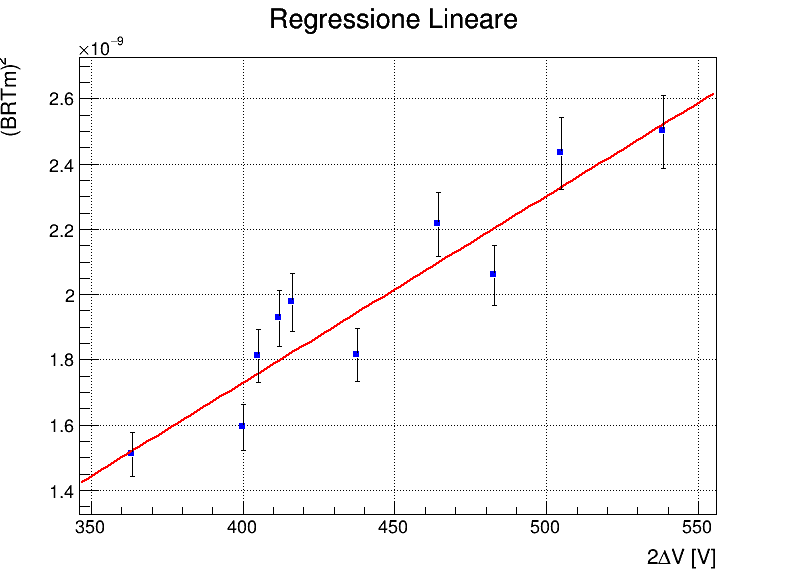
\includegraphics[width=0.6\textwidth]{regr_ortogonale.png}
        \caption{Regressione lineare in configurazione ortogonale.}
        \label{fig:regr_ortogonale}
    \end{figure}
    \textbf{Accordo}: \(3\%\) \\
    \textbf{Compatibilità}: \(95\%\)
    \vspace{0.5cm}

    \item \textbf{Configurazione Antiparallelo}: \( (1.79 \pm 0.20) \times 10^{11} \, \text{C/kg}\)
    \begin{figure}[H]
        \centering
        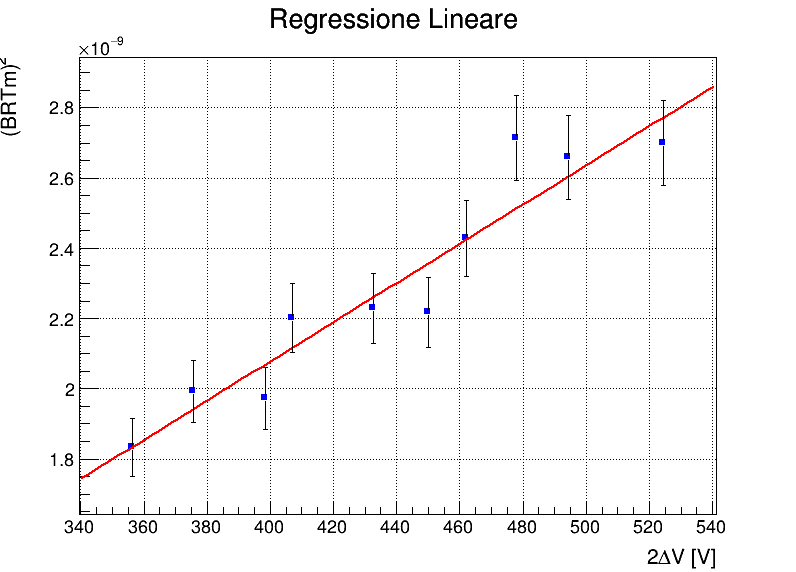
\includegraphics[width=0.6\textwidth]{regr_antiparallelo.png}
        \caption{Regressione lineare in configurazione antiparallelo.}
        \label{fig:regr_antiparallelo}
    \end{figure}
    \textbf{Accordo}: \(48\%\) \\
    \textbf{Compatibilità}: \(87\%\)
    \vspace{0.5cm}

    \item \textbf{Configurazione Parallelo}: \( (1.95 \pm 0.20) \times 10^{11} \, \text{C/kg}\)
    \begin{figure}[H]
        \centering
        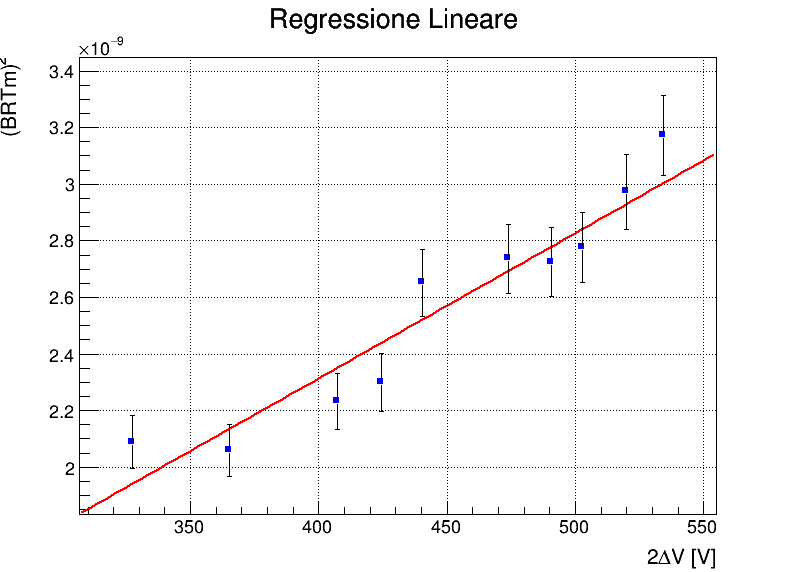
\includegraphics[width=0.6\textwidth]{regr_parallelo.png}
        \caption{Regressione lineare in configurazione parallelo.}
        \label{fig:regr_parallelo}
    \end{figure}
    \textbf{Accordo}: \(28\%\) \\
    \textbf{Compatibilità}: \(35\%\)
\end{itemize}
L’accordo del \(3\%\) dei punti sperimentali della misura nella configurazione perpendicolare con il modello teorico secondo cui i punti sperimentali debbano seguire un andamento lineare è ritenibile insoddisfacente (in quanto inferiore alla soglia convenzionale del \(5\%\)). Tuttavia, l’andamento lineare teorico è confermato con accordi ritenuti ampiamente accettabili, secondo la soglia percentuale di riferimento, nelle due regressioni lineari successive dove il test del \( \chi^2 \) produce un accordo del \(48\%\) e del \(28\%\).

% \begin{table}[H]
%     \centering
%     \begin{tabular}{|c|c|c|c|}
%         \hline
%         \textbf{Configurazione} & \(\frac{e}{m} \, (\text{C/kg})\) & \textbf{Accordo (\%)} & \textbf{Compatibilità (\%)} \\
%         \hline
%         Ortogonale & \( (1.75 \pm 0.23) \times 10^{11} \) & \( 31\% \) & \( 97\% \) \\
%         \hline
%         Parallelo & \( (1.79 \pm 0.27) \times 10^{11} \) & \( 83\% \) & \( 90\% \) \\
%         \hline
%         Antiparallelo & \( (1.95 \pm 0.27) \times 10^{11} \) & \( 71\% \) & \( 49\% \) \\
%         \hline
%     \end{tabular}
%     \caption{Misurazioni del rapporto carica-massa dell'elettrone}
%     \label{tab:em_measurements}
% \end{table}


\section{Misura del campo magnetico terrestre}

In seguito alle tre misurazioni del rapporto carica-massa dell’elettrone, si è condotta la misura della componente orizzontale del campo magnetico terrestre, attraverso l’apposito apparato.
Essendo inizialmente le bobine dell’apparato non alimentate da corrente, l’ago magnetico posizionato sulla piattaforma è orientato secondo la direzione e il verso della componente orizzontale del campo magnetico terrestre \( B_T \). Quindi, per prima cosa, si orienta l’apparato in modo che l’ago magnetico sia disposto lungo la direzione \( 0-180^\circ \) con un’incertezza di \( \pm 1^\circ \).
Nel momento in cui viene fatta scorrere corrente elettrica, di intensità impostabile tramite generatore, all’interno delle bobine, esse generano un campo magnetico, che risulta presentare:
\begin{itemize}
    \item una componente orizzontale \( B_z \), perpendicolare al campo magnetico terrestre, con verso invertibile tramite l’inversione del senso di corrente nelle bobine;
    \item una componente orizzontale \( B_r \), minore, nella stessa direzione del campo magnetico terrestre ma in verso opposto.
\end{itemize}

Il campo magnetico terrestre e quello delle bobine si sommano a generare un campo risultante \( B_{\text{TOT}} \), di diversa direzione rispetto al campo magnetico terrestre, da cui risulta separato angolarmente di un certo angolo \( \theta \), dipendente dal campo generato dalle bobine e quindi dall’intensità di corrente selezionata.
L’ago magnetico risente della variazione del campo magnetico allineandosi nella direzione e verso del nuovo campo magnetico risultante, ruotando quindi di un angolo pari a \( \theta \), in senso orario o antiorario in base al verso della corrente nelle bobine.

\subsection{Relazione tra i campi magnetici}
Schematizzando geometricamente i vettori in gioco, si osserva che, alla condizione di equilibrio dell'ago magnetico, vale la relazione:
\begin{equation}
    \tan \theta = \frac{B_z}{B_T - B_r}
    \label{eq:tan_theta}
\end{equation}
Da cui si ricava:
\begin{equation}
    B_T = B_z \cot \theta + B_r
    \label{eq:BT_formula}
\end{equation}
I valori di \( B_z \) e \( B_r \) dell’apparato utilizzato con una corrente di intensità \( I_0 = 100 \, \text{mA} \) sono tabulati al variare di \( \theta \), con incertezza trascurabile.
Impostando nelle bobine una corrente di intensità \( I \) per misurare un valore di \( \theta \) tabulato, cioè di cui sono noti i rispettivi valori di \( B_z \) e \( B_r \), si ottiene:
\begin{equation}
    B_T = \frac{I}{I_0} \left( B_z \cot \theta + B_r \right)
    \label{eq:BT_with_I}
\end{equation}

\subsection{Riduzione degli errori}
Per ridurre il possibile errore iniziale sul posizionamento dell’ago, per ogni angolo si inverte la direzione della corrente e, se necessario, si modifica \( I \), per ottenere lo stesso angolo specchiato rispetto all’origine. Infine, si effettua la media delle due intensità utilizzate.

\subsection{Incertezza sul campo magnetico terrestre}
L’incertezza sul valore del campo magnetico terrestre, a partire dall’incertezza sull’intensità di corrente delle bobine e sulla deviazione angolare dell’ago magnetico, si ottiene per propagazione degli errori:
\begin{equation}
    \sigma_{B_T} = \frac{1}{I_0} \sqrt{\left[ \left( B_z \cot \theta + B_r \right) \sigma_I \right]^2 + \left( I \frac{B_z}{\sin^2 \theta} \sigma_\theta \right)^2}
    \label{eq:sigma_BT}
\end{equation}

\subsection{Risultati sperimentali}
Sono state impostate 10 diverse intensità di corrente e sono stati misurati ogni volta i relativi spostamenti angolari dell’ago magnetico. Si sono dunque calcolati 10 valori del campo magnetico terrestre, con relativa incertezza, di cui si è calcolata la media pesata.

L’incertezza sistematica su ogni misura di intensità di corrente è stata stimata di \( 0.3 \, \text{mA} \), in base all’oscillazione del valore leggibile sul display dell’amperometro utilizzato, ed è stata ridotta di un fattore \( \sqrt{2} \) grazie alla media svolta con l’altro valore di intensità. D’altra parte, come incertezza sull’angolo di orientazione dell’ago magnetico si è stimata ragionevolmente \( 1^\circ \), tenendo conto dell’errore di parallasse.

Si è infine ottenuto una misura della componente orizzontale del campo magnetico terrestre a Milano pari a:
\[
    B_T = (24.6 \pm 0.4) \, \mu\text{T}
\]

\section{Conclusioni e correzioni}

Una volta determinata l’intensità della componente orizzontale del campo magnetico terrestre, è possibile correggere le misure del rapporto carica-massa dell’elettrone ottenute dalla conduzione dell’esperimento di Thompson nelle due configurazioni in cui il campo magnetico terrestre risulta, rispettivamente, parallelo e antiparallelo al campo magnetico generato dalle due bobine. 
Difatti, non considerando la presenza del campo magnetico terrestre nel caso in cui esso sia parallelo al campo delle bobine, si sottostima il campo magnetico che avvertono gli elettroni di cui è stato preso in esame il moto. Il che, in linea teorica, comporta che ci si attenda un valore sovrastimato del rapporto carica-massa dell’elettrone, per via della relazione:

\begin{equation}
    \frac{e}{m} = \frac{2 \Delta V}{B^2 R^2} \label{eq:em_relation}
\end{equation}

Difatti, la misura del rapporto carica-massa dell’elettrone nella configurazione parallela è risultata:

\[
(1.95 \pm 0.20) \times 10^{11} \, \text{C/kg}
\]
che sovrastima la misurazione perpendicolare:
\[
(1.75 \pm 0.17) \times 10^{11} \, \text{C/kg}
\]
e il valore accettato di:
\[
1.7588 \times 10^{11} \, \text{C/kg}.
\]

Analogamente, trascurando la presenza del campo magnetico terrestre nel caso in cui esso sia antiparallelo al campo generato dalle bobine, si arriva a sovrastimare il campo magnetico a cui sono soggetti gli elettroni. Ciò implica che ci si attenda un risultato sottostimato del rapporto carica-massa dell’elettrone. 

Si è pertanto stimata, con metodi statistici che coinvolgono la distribuzione gaussiana (che si ipotizza venga eseguita dalle misure effettuate in laboratorio), la compatibilità con l’eventualità che il valore misurato del rapporto carica-massa dell’elettrone nella configurazione antiparallela (in corrispondenza di cui si è ottenuta la misura):

\[
(1.79 \pm 0.20) \times 10^{11} \, \text{C/kg}
\]
sottostimi la misurazione perpendicolare 
\[
(1.75 \pm 0.17) \times 10^{11} \, \text{C/kg}
\]
e il valore vero
\[
1.7588 \times 10^{11} \, \text{C/kg}
\]
Ottenendo probabilità non trascurabili circa pari al \(43\%\).
Si nota come nel caso antiparallelo il valore misurato di e/m sia sovrastimato rispetto al valore di e/m nel caso perpendicolare, contraddicendo la teoria. Tuttavia, siccome nella prima misurazione si ottiene un range di valori \([1.75, 2.15] \times 10^{11}\text{C/kg}\), sempre superiore al valore perpendicolare, si può assumere con buona approssimazione che questa sia la configurazione parallela e di conseguenza la seconda misurazione antiparallela.
Si è quindi sommato il valore del campo magnetico terrestre ottenuto al campo delle bobine nel caso di configurazione parallela, e lo si è invece sottratto nel caso della configurazione antiparallela:

\begin{align}
    B_{\text{TOT}, \parallel} &= B_{\text{Bobine}} + B_T \label{eq:B_tot_parallel} \\
    B_{\text{TOT}, \text{anti}\parallel} &= B_{\text{Bobine}} - B_T \label{eq:B_tot_antiparallel}
\end{align}

L’incertezza sul campo magnetico risultante è ottenibile mediante somma in quadratura dell’incertezza sul campo magnetico generato dalle bobine, precedentemente determinata, e quella del campo magnetico terrestre, anch’essa determinata precedentemente:

\begin{equation}
    \sigma_{B_{\text{TOT}}} = \sqrt{\sigma_{B_{\text{Bobine}}}^2 + \sigma_{B_T}^2} \label{eq:B_tot_uncertainty}
\end{equation}

Rieffettuando le regressioni relative a queste due configurazioni, si ottiene, come previsto dalla formula, un aumento del valore ottenuto del rapporto carica-massa dell’elettrone nel caso di configurazione antiparallela, e una diminuzione del valore ottenuto del rapporto carica-massa dell’elettrone nel caso di configurazione parallela.

Di seguito i risultati ottenuti senza trascurare il campo magnetico terrestre nelle configurazioni parallelo e antiparallelo:

\begin{itemize}
    % \item \textbf{Configurazione Ortogonale}: \( (1.75 \pm 0.17) \times 10^{11} \, \text{C/kg}\)
    % \begin{figure}[H]
    %     \centering
    %     \includegraphics[width=0.6\textwidth]{.png}
    %     \caption{Regressione lineare in configurazione ortogonale.}
    %     \label{fig:correz_regr_ortogonale}
    % \end{figure}
    % \textbf{Accordo}: \(3\%\) \\
    % \textbf{Compatibilità}: \(95\%\)
    % \vspace{0.5cm}

    \item \textbf{Configurazione Antiparallelo}: \( (1.84 \pm 0.20) \times 10^{11} \, \text{C/kg}\)
    \begin{figure}[H]
        \centering
        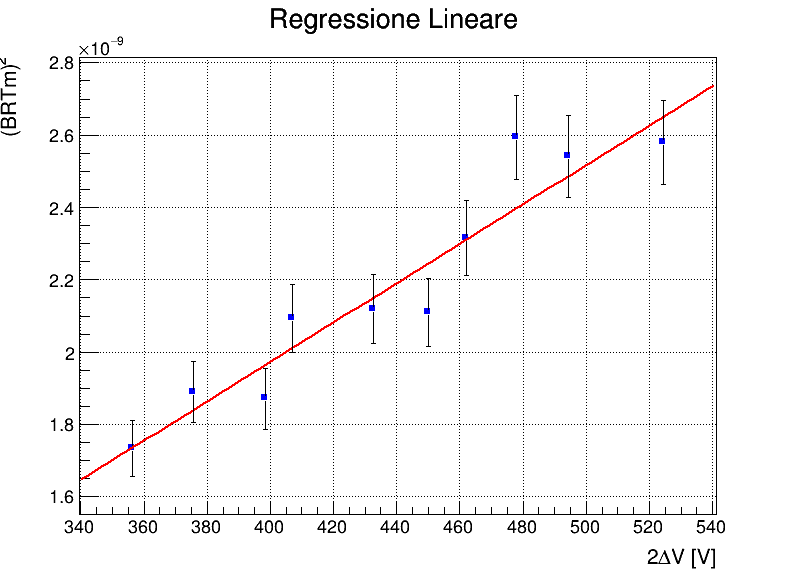
\includegraphics[width=0.6\textwidth]{correz_regr_antiparallelo.png}
        \caption{Regressione lineare in configurazione antiparallelo.}
        \label{fig:correz_regr_antiparallelo}
    \end{figure}
    \textbf{Accordo}: \(44\%\) \\
    \textbf{Compatibilità}: \(70\%\)
    \vspace{0.5cm}

    \item \textbf{Configurazione Parallelo}: \( (1.90 \pm 0.20) \times 10^{11} \, \text{C/kg}\)
    \begin{figure}[H]
        \centering
        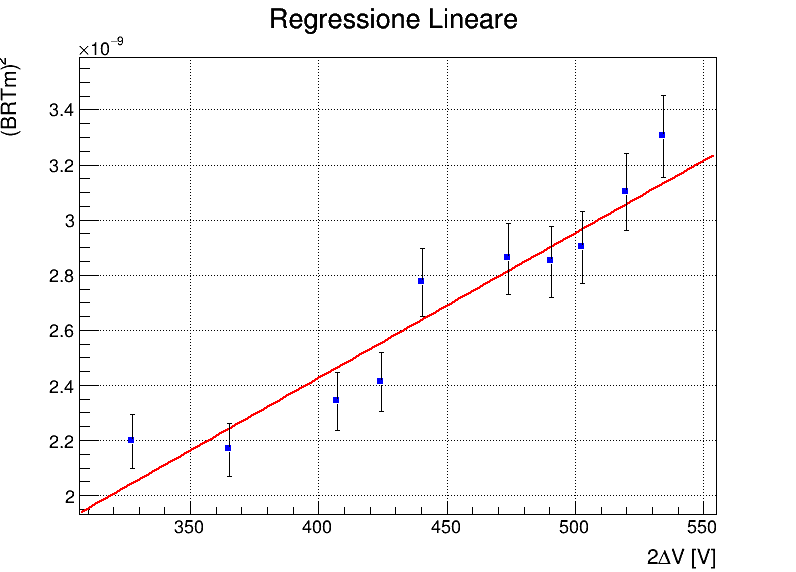
\includegraphics[width=0.6\textwidth]{correz_regr_parallelo.png}
        \caption{Regressione lineare in configurazione parallelo.}
        \label{fig:correz_regr_parallelo}
    \end{figure}
    \textbf{Accordo}: \(32\%\) \\
    \textbf{Compatibilità}: \(48\%\)
\end{itemize}
Si noti come la compatibilità, con il valore del valore accettato, della misura nella configurazione parallela del rapporto carica-massa elettrone aumenti, passando dal \(35\%\) al \(48\%\), in seguito alla correzione del campo magnetico terrestre che produce una diminuzione il valore sovrastimato. 

\end{document}